\documentclass[margin=0.1cm]{standalone}

%\usepackage{stix2}
\usepackage[]{tgheros}
\renewcommand{\familydefault}{\sfdefault}
\usepackage{arevmath}
\usepackage[italic]{mathastext}
\usepackage[T1]{fontenc}

\usepackage{pgfplots}
\pgfplotsset{compat=1.17}
\usepackage{siunitx}

\usepackage{booktabs}

\begin{document}
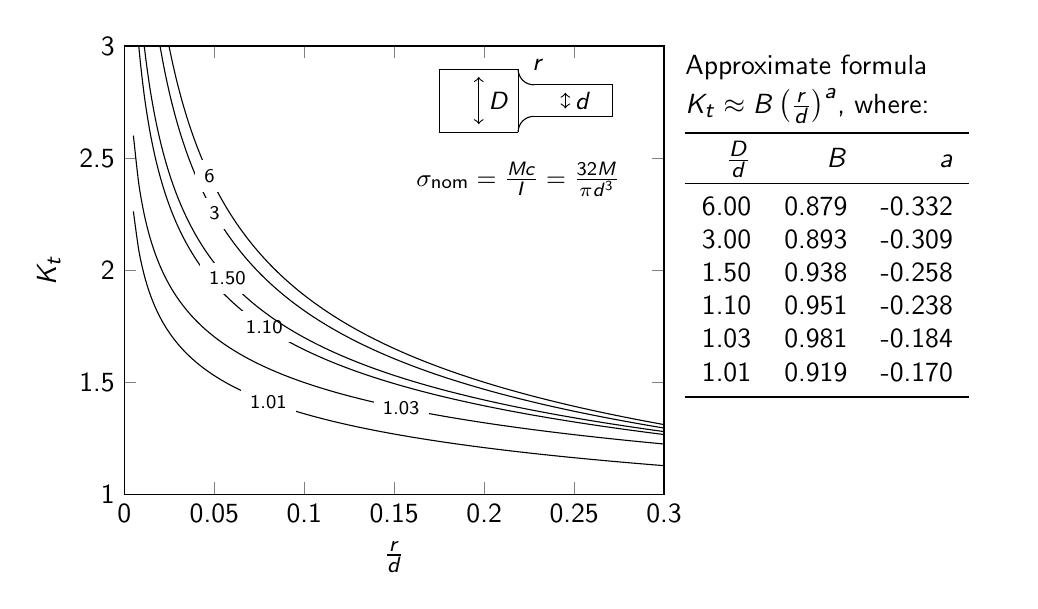
\begin{tikzpicture}
    \begin{axis}[
        xlabel = $\frac{r}{d}$,
        ylabel = $K_t$,
        ymin={1},
        ymax={3},
        xmin={0},
        xmax={0.3},
        x tick label style={
            /pgf/number format/.cd,
                fixed,
                %fixed zerofill,
                precision=2,
            /tikz/.cd
        },
        domain={0.005:0.3},
        samples={100}
    ]
    
    \addplot[smooth] {0.919*x^-0.170} node[pos=0.7, fill=white] {\scriptsize 1.01};
    \addplot[smooth] {0.981*x^-0.184} node[pos=0.85, fill=white] {\scriptsize 1.03};
    \addplot[smooth] {0.951*x^-0.238} node[pos=0.75, fill=white] {\scriptsize 1.10};
    \addplot[smooth] {0.938*x^-0.258} node[pos=0.7, fill=white] {\scriptsize 1.50};
    \addplot[smooth] {0.893*x^-0.309} node[pos=0.7, fill=white] {\scriptsize 3};
    \addplot[smooth] {0.879*x^-0.332} node[pos=0.7, fill=white] {\scriptsize 6};
    
    \end{axis}
    
    %% Drawing (going clockwise from top left)
    
    \draw[] (4,5.4) -- (5,5.4);
    \draw (5,5.4) arc [start angle=180, end angle=270, x radius=0.2cm, y radius=0.2cm] node[pos=0.5, anchor=south west] {\small $r$};
    \draw[] (5.2,5.2) -- (6.2, 5.2);
    \draw[] (6.2,5.2) -- (6.2, 4.8);
    \draw[] (6.2,4.8) -- (5.2, 4.8);
    \draw (5,4.6) arc [start angle=180, end angle=90, x radius=0.2cm, y radius=0.2cm];
    \draw[] (5.0,4.6) -- (4.0, 4.6);
    \draw[] (4.0, 4.6) -- (4, 5.4);
    
    \draw[] (5.0, 4.6) -- (5.0, 5.4);
    
    \draw[<->] (4.5, 4.7) -- (4.5, 5.3) node[pos=0.5, anchor=west] {\small $D$};
    
    \draw[<->] (5.6, 4.9) -- (5.6, 5.1) node[pos=0.5, anchor=west] {\small $d$};

    \node[] at (5, 4) (maths) {\small$\sigma_\text{nom}=\frac{Mc}{I}=\frac{32M}{\pi{}d^3}$};
    
    %% Table %%
    
    \node[anchor=north west, text width=4cm] at (7, 5.7) (table) {
        Approximate formula \\[0.2em]
        $K_t\approx B\left(\frac{r}{d}\right)^a$, where:\\[0.2em]
        \begin{tabular}{rrr}
            \toprule
            $\frac{D}{d}$ & $B$ & $a$ \\
            \midrule
            6.00 & 0.879 & -0.332 \\
            3.00 & 0.893 & -0.309 \\
            1.50 & 0.938 & -0.258 \\
            1.10 & 0.951 & -0.238 \\
            1.03 & 0.981 & -0.184 \\
            1.01 & 0.919 & -0.170 \\
            \bottomrule
        \end{tabular}
    };
\end{tikzpicture}
\end{document}